\section{Arquitectura del nuevo modelo híbrido}

\subsection{ Motivación y diferencias respecto a la SNN original}

La motivación principal para desarrollar este modelo híbrido surge de las limitaciones observadas en la SNN original. Esta red se diseñó para procesar series temporales de datos (como los datasets de IoPS o CalIt2) mediante un enfoque de aprendizaje no supervisado basado en \textbf{STDP}, con el objetivo de detectar anomalías a través de patrones de disparos neuronales. Sin embargo, su estructura fully-connected limita la capacidad para capturar dependencias temporales y espaciales complejas en los datos, lo que resulta en un rendimiento subóptimo en escenarios con ruido o variabilidad alta. Además, carece de mecanismos de optimización sistemática de hiperparámetros y de procesamiento jerárquico, lo que puede llevar a sobreajuste o baja generalización.

\textbf{Resumen de la arquitectura previa (A--B, 39 LIF + 100 LIF) y sus limitaciones:}

La SNN original consta de dos capas principales:
\begin{itemize}
    \item \textbf{Capa de entrada (A)}: Compuesta por un número variable de neuronas de entrada (típicamente $\sim$39, determinado por el tamaño de los cuantiles derivados de los datos de entrenamiento, \texttt{snn\_input\_layer\_neurons\_size = len(cuantiles)-1}). Estas neuronas codifican los valores de la serie temporal en impulsos (spikes) basados en rangos cuantificados.
    \item \textbf{Capa de procesamiento (B)}: Formada por 100 neuronas LIF (Leaky Integrate-and-Fire, \texttt{snn\_process\_layer\_neurons\_size = 100}), conectadas de manera fully-connected a la capa A. Utiliza aprendizaje STDP con tasas de aprendizaje \texttt{nu1} y \texttt{nu2} para ajustar pesos sinápticos. La red se entrena exponiendo secuencias de datos durante un tiempo \texttt{T} (e.g., 100), y los disparos en B se usan para inferir anomalías (e.g., mediante umbrales como \texttt{umbral\_anomalia = np.mean(spikes) + 2 * np.std(spikes)}).
\end{itemize}

Limitaciones clave:
\begin{itemize}
    \item \textbf{Falta de extracción de características jerárquicas}: La conexión fully-connected no captura patrones locales o temporales de manera eficiente, lo que es crítico en series temporales con anomalías sutiles (e.g., picos o cambios graduales).
    \item \textbf{Sensibilidad a hiperparámetros}: Valores fijos o manuales para \texttt{nu1}, \texttt{nu2}, \texttt{threshold} y \texttt{decay} limitan la adaptabilidad, sin optimización automatizada.
    \item \textbf{Rendimiento en datasets ruidosos}: En datasets como IoPS, la red puede generar falsos positivos debido a la ausencia de procesamiento convolucional para filtrar ruido temporal.
    \item \textbf{Eficiencia computacional}: No incorpora capas especializadas para reducir dimensionalidad, lo que aumenta el costo en datasets grandes.
    \item \textbf{Criterio de alerta simple}: Basado únicamente en estadísticas de disparos en B (e.g., suma de spikes > umbral), sin rutas alternativas para refinamiento.
\end{itemize}

El nuevo modelo híbrido aborda estas limitaciones integrando una capa convolucional (C) después de B, creando una arquitectura híbrida (SNN + convolucional). Esto permite una extracción de características más robusta, similar a las CNN tradicionales, pero adaptada a spikes. La motivación es mejorar la detección de anomalías en series temporales mediante:
\begin{itemize}
    \item \textbf{Procesamiento jerárquico}: La capa C aplica convoluciones sobre los disparos de B para capturar patrones locales (usando kernels gaussiano).
    \item \textbf{Optimización con Optuna}: Hiperparámetros se optimizan automáticamente para maximizar métricas como F1-score.
    \item \textbf{Rutas duales de datos}: Permite procesar salidas de B y C en paralelo, con criterios de alerta basados en MSE y métricas de clasificación.
    \item \textbf{Mejora en generalización}: Soporte para datasets como IoPS y CalIt2, con expansión de etiquetas y padding para manejar secuencias variables.
\end{itemize}

Diferencias clave incluyen la adición de monitores para la capa C (\texttt{conv\_monitor}), opciones de procesamiento convolucional (e.g., 'weighted\_sum' o 'max'), y métricas duales (para B y C). Esto resulta en un modelo más flexible y efectivo, con un F1-score potencialmente superior en pruebas.


\subsection{Análisis de Variables Modificables del Modelo Híbrido}

\textbf{Tabla comparativa de cambios estructurales:}

Estas tablas (\ref{tab:comparacion-arquitecturas-1} y \ref{tab:comparacion-arquitecturas-2})  resalta cómo el modelo híbrido extiende la original sin alterar su núcleo, pero modificando donde es necesario para mejorar el rendimiento.

\begin{table}[!htbp]
\centering
\small
\renewcommand{\arraystretch}{1.3}
\begin{tabularx}{0.99\textwidth}{>{\hsize=0.5\hsize\raggedright\arraybackslash}X
                                 >{\hsize=1.2\hsize\raggedright\arraybackslash}X
                                 >{\hsize=1.3\hsize\raggedright\arraybackslash}X}
\hline\hline
\textbf{Aspecto} & \textbf{SNN Original (A--B)} & \textbf{Modelo Híbrido (A--B--C)} \\
\hline
\textbf{Tipo de capas} & 
A: Input (codificación de cuantiles).  

B: Fully-connected LIF. & 

A: Input (codificación de cuantiles).  

B: Fully-connected LIF con conexiones recurrentes.  

C: AdaptiveLIF con kernels convolucionales configurables (Gaussian, Laplacian, Mexican Hat, Box). \\
\hline
\textbf{Número Neuronas} & 
A: Variable según cuantiles (\texttt{len(cuantiles)-1}).

B: 100 (fijo). & 

A: Variable según cuantiles (\texttt{len(cuantiles)-1}).  

B: Configurable vía \texttt{snn\_process\_layer\_neurons\_size} (por defecto: 100).  

C: Igual tamaño que B (\texttt{n = snn\_process\_layer\_neurons\_size}). \\
\hline
\textbf{Conexiones} & 
A $\rightarrow$ B: Pesos aleatorios.  

B $\rightarrow$ B: Recurrentes con pesos negativos. & 

A $\rightarrow$ B: Pesos \texttt{0.3 + 0.2*randn}.

B $\rightarrow$ B: Recurrentes \texttt{0.025*(eye-1)}.

B $\rightarrow$ C: Convolucional con kernels optimizables. \\
\hline
\textbf{Parámetros Optimizables} & 
Parámetros fijos o manuales:  
\texttt{nu1}, \texttt{nu2}, \texttt{threshold}, \texttt{decay}. & 
Optimización vía Optuna:  

\texttt{nu1}, \texttt{nu2} $\in$ [-0.5, 0.5].

\texttt{threshold} $\in$ [-65, -50].  

\texttt{decay} $\in$ [80, 150].  

\texttt{kernel\_size} $\in$ [3, 9] (impares).  

\texttt{sigma} $\in$ [0.5, 3.0].  

\texttt{norm\_factor} $\in$ [0.1, 1.0].  

\texttt{exc\_inh\_balance} $\in$ [-0.3, 0.3]. \\
\hline
\textbf{Procesamiento Convolucional} & 
No disponible. & 
Tres modos: \texttt{direct}, \texttt{weighted\_sum}, \texttt{max}.  
Kernels adaptativos con balance excitatorio-inhibitorio. \\
\hline\hline
\end{tabularx}
\caption{Comparación entre SNN original y modelo híbrido — Parte 1: arquitectura, conexiones y optimización.}
\label{tab:comparacion-arquitecturas-1}
\end{table}

\begin{table}[!htbp]
\centering
\small
\renewcommand{\arraystretch}{1.3}
\begin{tabularx}{0.99\textwidth}{>{\hsize=0.5\hsize\raggedright\arraybackslash}X
                                 >{\hsize=1.2\hsize\raggedright\arraybackslash}X
                                 >{\hsize=1.3\hsize\raggedright\arraybackslash}X}
\hline\hline
\textbf{Aspecto} & \textbf{SNN Original (A--B)} & \textbf{Modelo Híbrido (A--B--C)} \\
\hline
\textbf{Criterio de alerta} & 
Basado en umbral estadístico en spikes de B.  
Métricas: Precisión, Recall, F1. & 
Evaluación dual: Spikes de B y C.  
Optimización: Maximiza \texttt{max(F1\_B, F1\_C)}.  
Métricas: MSE, F1, Precisión, Recall para ambas capas. \\
\hline
\textbf{Integración con MLOps} & 
Sin integración automatizada. & 
Integración con Weights \& Biases (wandb).  
Seguimiento de experimentos y métricas en tiempo real.  
Guardado automático de configuraciones óptimas. \\
\hline
\textbf{Dispositivo de Cómputo} & 
CPU únicamente. & 
Soporte para CPU/GPU configurable.  
Optimización automática según disponibilidad de hardware. \\
\hline
\textbf{Limitaciones abordadas} & 
Sensible a ruido; parámetros fijos; sin extracción de características locales. & 
Reducción de ruido vía convolución adaptativa.  
Optimización automática de hiperparámetros.  
Extracción de patrones temporales mejorada.  
Escalabilidad en hardware. \\
\hline\hline
\end{tabularx}
\caption{Comparación entre SNN original y modelo híbrido — Parte 2: evaluación, implementación y ventajas.}
\label{tab:comparacion-arquitecturas-2}
\end{table}


\subsection{Variables Centrales del Modelo Híbrido}

\subsection{Parámetros de Optimización con Optuna}

\subsubsection*{Parámetros de Aprendizaje STDP}

\begin{itemize}
    \item \textbf{nu1}: Controla la actualización sináptica en la conexión A→B (entrada a procesamiento).
    \item \textbf{nu2}: Regula el aprendizaje en conexiones B→B (recurrentes) y B→C (convolucionales).
\end{itemize}

 Valores negativos fortalecen conexiones (excitación), valores positivos las debilitan (inhibición). El rango [-0.5, 0.5] permite explorar desde inhibición fuerte hasta excitación moderada.

\subsubsection*{Parámetros Neuronales LIF}

\begin{itemize}
    \item \textbf{threshold}:  Umbral de disparo de las neuronas LIF/AdaptiveLIF. Umbrales más altos (-50 mV) requieren mayor activación para disparar, creando mayor selectividad.
    \item \textbf{decay}: Constante de tiempo de decaimiento de la membrana neuronal. Decaimientos altos (150) mantienen la información por más tiempo.
\end{itemize}


\subsubsection{Configuración de Parámetros Convolucionales del Kernel}


\begin{itemize}
    \item \textbf{kernel\_type}: Define la forma del filtro convolucional.
    
    \textbf{Gaussian}: Suavizado gradual, ideal para reducir ruido temporal
   
    \textbf{Laplacian}: Detección de bordes/cambios abruptos.

    \textbf{Mexican Hat}: Detección de características con supresión lateral.

    \textbf{Box}: Promediado simple, computacionalmente eficiente.
    
    \item \textbf{kernel\_size}: Tamaño de la ventana temporal del filtro (solo valores impares). 
    Valores pequeños (3): Capturan cambios rápidos, mayor sensibilidad
Valores grandes (9): Suavizado temporal extenso, menor sensibilidad al ruido
    \item \textbf{sigma}: Anchura del filtro gaussiano.
    Valores bajos (0.5): Kernels más puntiagudos, filtrado local
Valores altos (3.0): Kernels más anchos, filtrado global
\end{itemize}

\subsubsection{Balance Excitatorio-Inhibitorio}

\begin{itemize}
    \item \textbf{norm\_factor}: Factor de normalización de pesos convolucionales. Controla la intensidad global de las conexiones B→C. Valores altos (1.0) aumentan la influencia de la capa convolucional.
    \item \textbf{exc\_inh\_balance}: Balance entre conexiones excitatorias/inhibitorias. Implementado mediante máscara aleatoria en la matriz de pesos. Valores negativos (-0.3): Predominan conexiones inhibitorias. Valores positivos (0.3): Predominan conexiones excitatorias.
\end{itemize}

\subsection{Modos de Procesamiento Convolucional}


% Modalidades de Fusión
% direct: Usa directamente los spikes de la capa C

% Python
% conv_spikes = spikes["C"].float().sum(dim=2).transpose(0, 1)
% weighted_sum: Combinación ponderada de capas B y C

% Python
% conv_spikes = 0.3 * b_spikes_sum + 0.7 * c_spikes_sum
% Mayor peso (0.7) a la capa convolucional, aprovechando el filtrado
% max: Elemento máximo entre ambas capas

% Python
% conv_spikes = torch.maximum(b_spikes_sum, c_spikes_sum)
% Preserva la activación más fuerte, útil para detección de anomalías


\begin{itemize}
    \item \textbf{direct}:
        \begin{lstlisting}
            conv\_spikes = spikes[C].float().sum(dim=2).transpose(0, 1)
        \end{lstlisting}
        
        Usa directamente los spikes de la capa \textbf{C}
    \item \textbf{weighted\_sum}:
        \begin{lstlisting}
            conv\_spikes = 0.3 * b\_spikes\_sum + 0.7 * c\_spikes\_sum
        \end{lstlisting}
        
        Combinación ponderada de capas \textbf{B} y \textbf{C}. Mayor peso (0.7) a la capa convolucional, aprovechando el filtrado.
    \item \textbf{max}:
        \begin{lstlisting}
            conv\_spikes = torch.maximum(b\_spikes\_sum, c\_spikes\_sum)
        \end{lstlisting}
        
        Elemento máximo entre ambas capas. Preserva la activación más fuerte, útil para detección de anomalías.
\end{itemize}

% \subsection{Parámetros Temporales y de Codificación}


% T: Determina la duración de simulación por secuencia
% Mayor T permite mayor integración temporal pero aumenta el costo computacional
% expansion: Amplifica la representación de anomalías en los datos de entrenamiento
% Crítico para balancear clases en datasets desbalanceados

% \begin{itemize}
%     \item \textbf{T}: Tiempo por secuencia (simulación).
%     \item \textbf{expansion}: Amplificación de etiquetas anómalas.
%     \item \textbf{a}, \textbf{r}: Parámetros de cuantiles.
% \end{itemize}

% \subsection{Matriz de Pesos Convolucional}

% \begin{lstlisting}
% weights = torch.zeros(n, n, device=device)
% center = kernel_size // 2
% for offset in range(-center, center + 1):
%     cols = torch.clamp(rows + offset, 0, n - 1)
%     kernel_idx = offset + center
%     weights[rows, cols] = kernel_values[kernel_idx]
% \end{lstlisting}

% \noindent Esta implementación en forma de matriz de Toeplitz preserva la estructura local en el filtrado.

% \subsection{Conexiones de Retroalimentación}

% \begin{lstlisting}
% feedback_connection = Connection(
%     source=conv_layer,
%     target=target_layer,
%     w=0.05 * torch.randn(n, n, device=device),
%     update_rule=PostPre,
%     nu=nu2_value * 0.5
% )
% \end{lstlisting}

% \noindent Esta conexión permite modulación desde la capa convolucional hacia la base, habilitando refinamiento jerárquico.

% \subsection{Criterio de Optimización Dual}

% \begin{lstlisting}
% best_f1 = max(f1_B if f1_B is not None else 0, f1_C if f1_C is not None else 0)
% return -best_f1
% \end{lstlisting}

% \noindent El modelo selecciona automáticamente la mejor representación (B o C) basada en el \textit{F1-score}.

% \section*{Conclusión}

% El modelo híbrido representa un avance sustancial respecto a arquitecturas SNN tradicionales, integrando capacidades convolucionales, aprendizaje no supervisado y optimización dinámica mediante Optuna. Esta flexibilidad lo convierte en una herramienta poderosa para la detección de anomalías en series temporales complejas.    
    
\subsection{Esquema general}

A continuación se presenta el esquema global de la arquitectura híbrida SNN–CNN, integrando tres dominios diferenciados: \textbf{codificación y preprocesado}, \textbf{arquitectura SNN} (capas A,B) y bloque convolucional híbrido (capa C). El diagrama muestra cómo fluye la información desde la señal de entrada hasta la inferencia final, destacando las rutas paralelas de procesamiento y los puntos de monitorización clave.

En el primer dominio, la señal de serie temporal es previamente procesada y codificada en impulsos espiga (spikes) a través de cuantización y batching temporal. Este bloque prepara los trenes de spikes que alimentan el núcleo SNN. A continuación, en el segundo dominio, la capa A recibe estas espigas y las transmite a la capa B, donde se aplica dinámica recurrente LIF con aprendizaje STDP. La salida de B se bifurca: una ruta va directamente a la fase de inferencia sobre spikes de B, y la otra alimenta el bloque convolucional.

El tercer dominio corresponde a la capa C, que aplica convoluciones 1D sobre los spikes de la capa B utilizando kernels configurables (Gaussianos, Laplacianos, etc.). Esta capa aporta filtrado adaptativo y extracción de características locales antes de enviar su salida al mecanismo de decisión dual. Finalmente, el sistema evalúa ambas rutas (B y C) según métricas de clasificación y MSE, seleccionando automáticamente la representación más informativa.

% La figura ilustra de forma unificada este flujo de datos y las interfaces entre bloques. Más adelante, cada sección del diagrama será ampliada (“zoom in”) para detallar su funcionamiento interno y su correspondencia con los apartados específicos de este documento.

\begin{figure}[!htb]
    \centering
    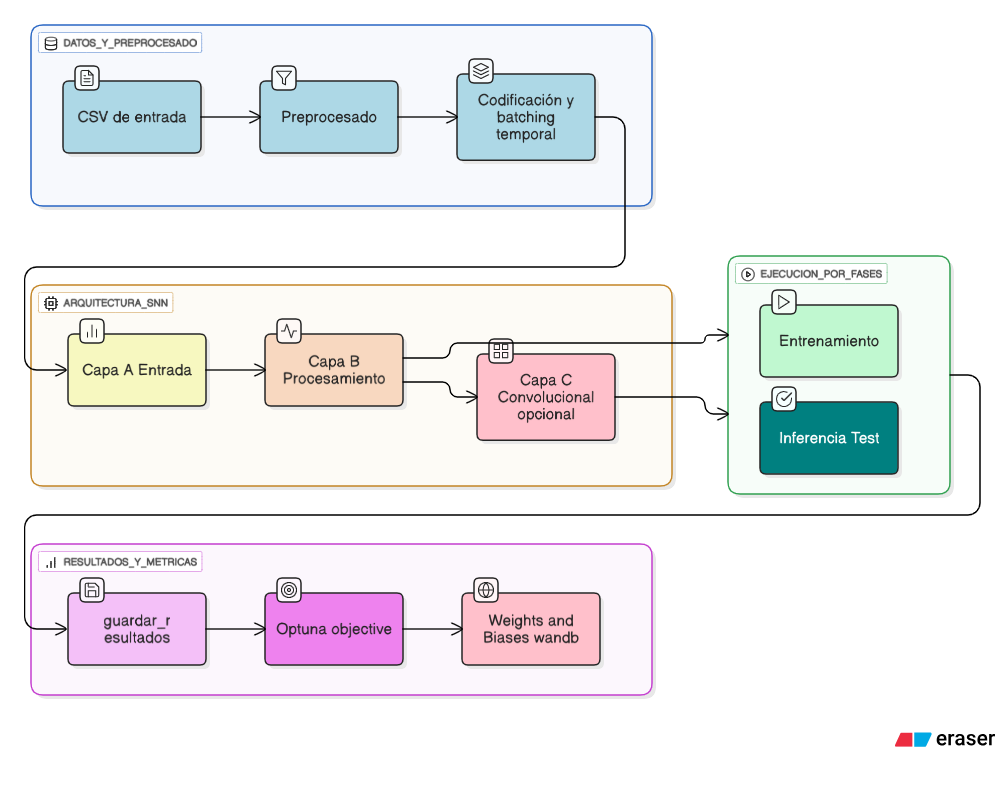
\includegraphics[width=1.0\textwidth]{Imagenes/Diagrama SNN.png}
    \caption{Flujo de datos y arquitectura SNN. Fuente: Elaboración propia.}
    \label{fig:Flujo de datos y arquitectura SNN}
\end{figure}

\subsubsection{Codificación y preprocesado de la señal}

En este bloque inicial la serie temporal bruta se divide en conjuntos de entrenamiento y prueba, se reinician los índices y se expanden las etiquetas para balancear clases. A continuación, se calculan los valores mínimos, máximos y cuantiles sobre el conjunto de entrenamiento, determinando el número de neuronas de la capa A. Finalmente, los datos se fragmentan en secuencias de longitud T y se aplica padding al conjunto de prueba para ajustarlo a múltiplos de T. Esta cadena de operaciones garantiza que las entradas al modelo estén normalizadas, codificadas por cuantiles y empaquetadas en batches temporales listos para generar trenes de spikes.

\begin{figure}[!htb]
    \centering
    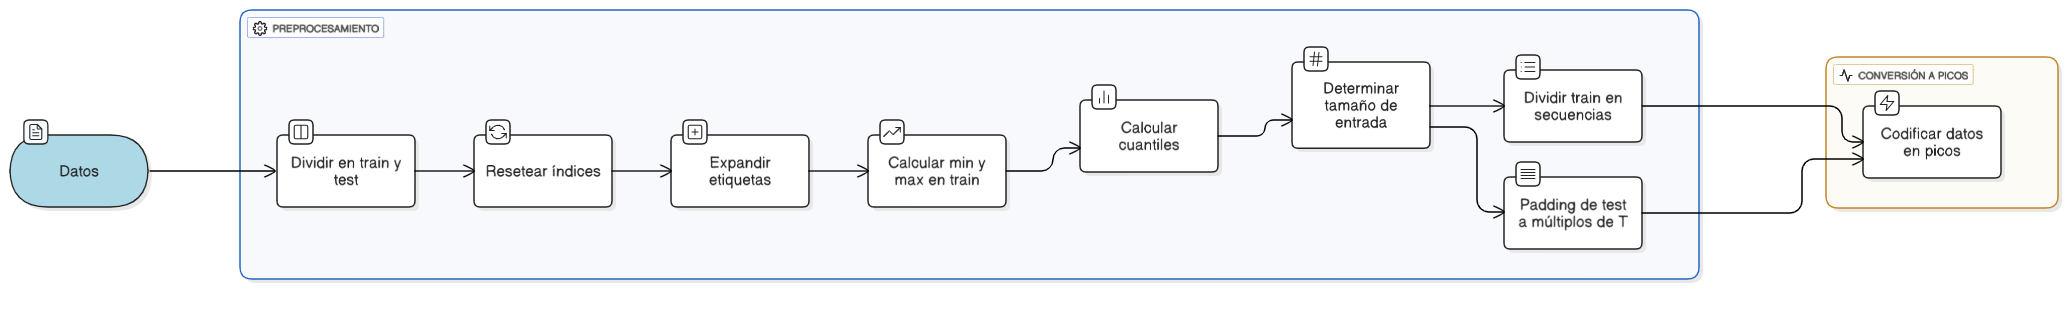
\includegraphics[width=1.0\textwidth]{Imagenes/Codificación y preprocesado de la señal (2).png}
    \caption{Codificación y preprocesado de la señal. Fuente: Elaboración propia.}
    \label{fig:Codificación y preprocesado de la señal}
\end{figure}
    
% \subsection{Codificación y preprocesado de la señal}
% 	•	Binarización revisada (rangos dinámicos y quantiles).
% 	•	Mecanismo de empaquetado de secuencias para convolución posterior.



    
% \subsection{Bloque SNN base}
% 	•	Configuración de las capas A y B (tamaños, recurrentes, parámetros LIF).
% 	•	Regla STDP modificada (ν = 0.1, doble penalización) y su impacto sobre sparsity.
    
\subsection{Capa convolucional híbrida (SNN-CNN)}

La incorporación de una capa convolucional híbrida representa una de las innovaciones más significativas del modelo propuesto, fusionando la eficiencia energética de las SNNs con las capacidades de extracción de características espaciales de las redes neuronales convolucionales. Esta arquitectura híbrida surge tras una exhaustiva exploración de múltiples configuraciones arquitecturales, buscando optimizar tanto el rendimiento predictivo como la viabilidad computacional.

\subsubsection {Posicionamiento arquitectural}

La capa convolucional híbrida se posiciona estratégicamente después de la \textbf{capa B} de procesamiento, recibiendo directamente los trenes de spikes generados por las neuronas LIF recurrentes. Esta ubicación permite que la capa procese patrones temporales ya refinados por la dinámica recurrente de la SNN base, aprovechando la información codificada en los tiempos de disparo de los spikes.

La decisión arquitectural de posicionar la capa convolucional en este punto específico se fundamenta en evidencia experimental que demuestra que las arquitecturas híbridas SNN-CNN alcanzan un rendimiento superior cuando combinan el procesamiento temporal asíncrono de las SNNs con las operaciones de convolución espacial \cite{sanaullah_hybrid_2024}. Esta configuración permite que los trenes de spikes de la capa B mantengan su estructura temporal intrínseca mientras son procesados por kernels convolucionales especializados.

\subsubsection{Detalle arquitectural de la capa convolucional híbrida}

\begin{figure}[!htb]
    \centering
    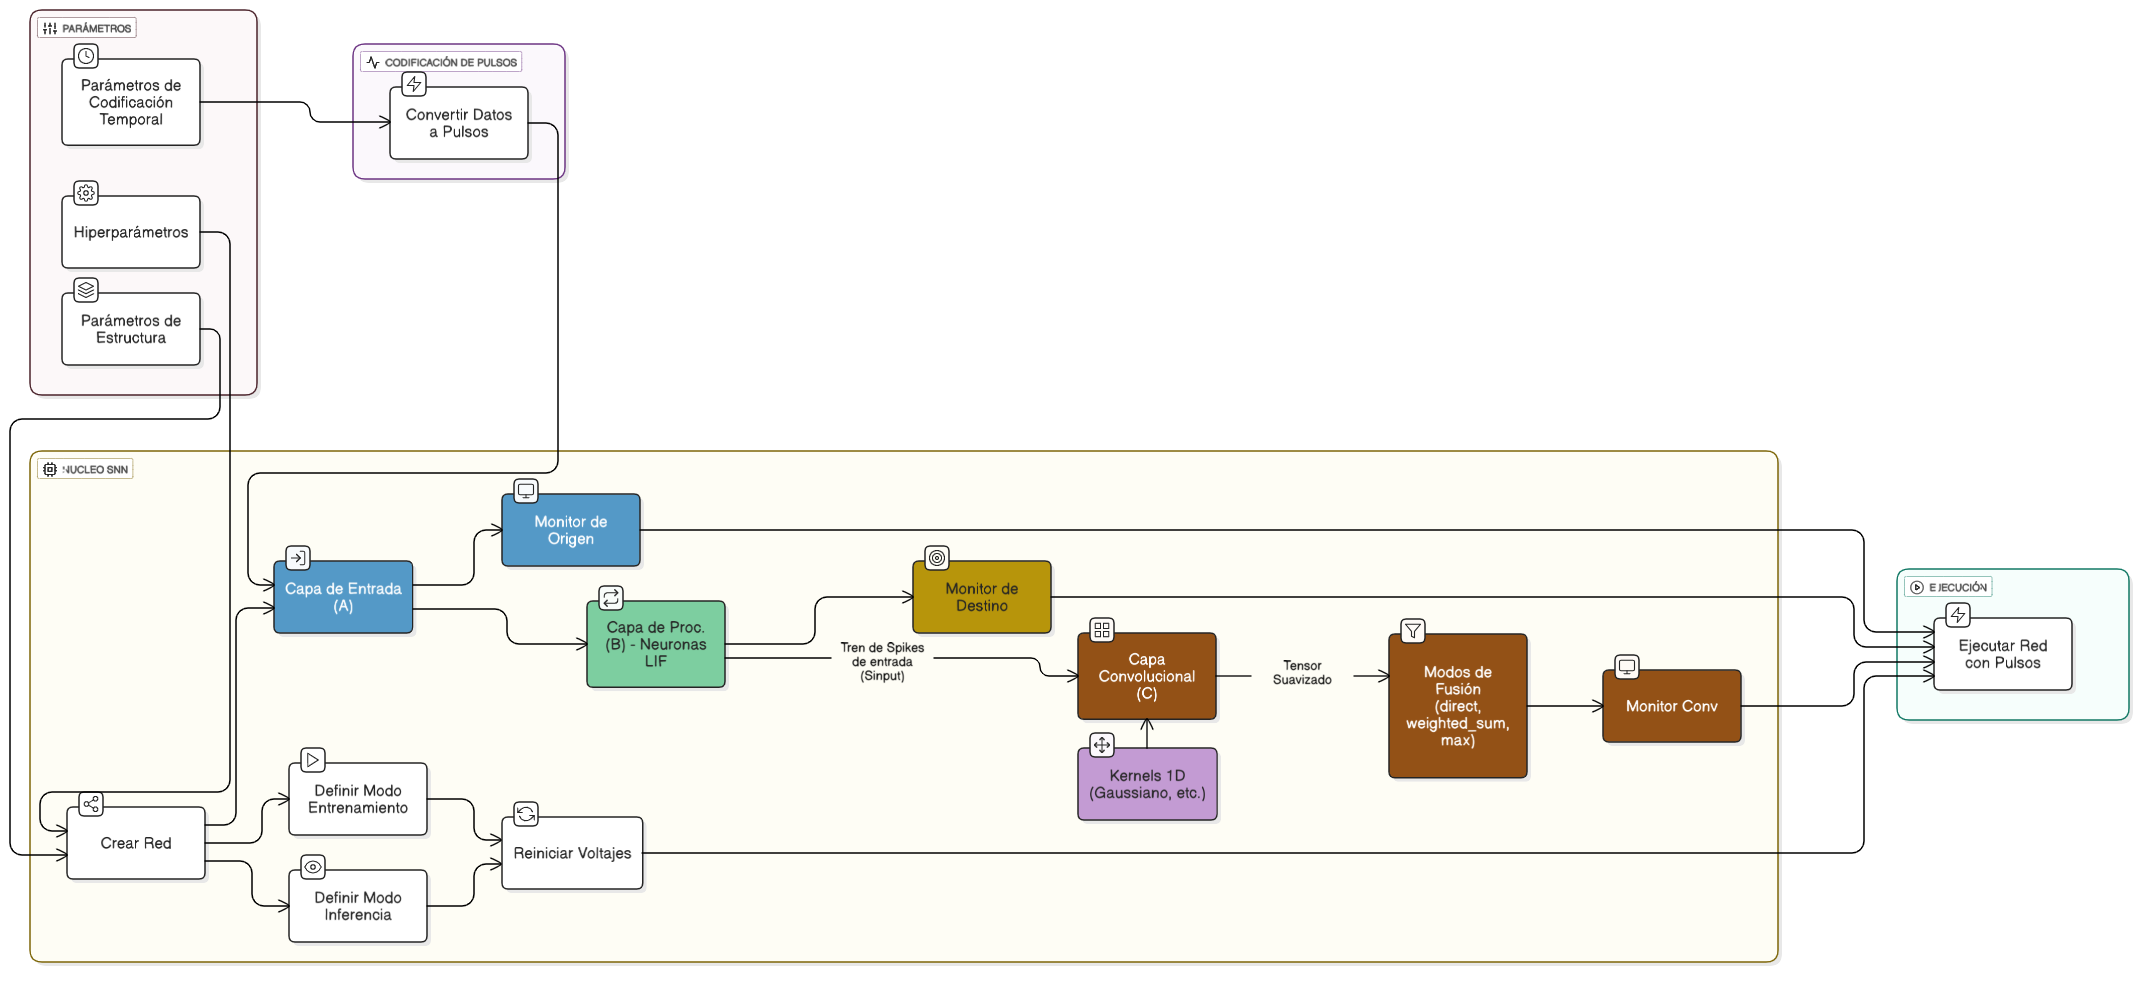
\includegraphics[width=1.0\textwidth]{Imagenes/Arquitectura detallada SNN.png}
    \caption{Arquitectura detallada de la capa convolucional híbrida mostrando el flujo desde los spikes de la capa B hacia el procesamiento convolucional con kernels adaptativos. Fuente: Elaboración propia.}
    \label{fig:Arquitectura detallada SNN}
\end{figure}

La figura \ref{fig:Arquitectura detallada SNN} ilustra el flujo específico de procesamiento dentro del núcleo SNN, destacando cómo los trenes de spikes generados por las neuronas LIF de la capa B son procesados por kernels convolucionales especializados antes de generar las salidas de la capa C. Este procesamiento incluye la aplicación de diferentes tipos de kernels (Gaussiano, Laplaciano, etc.) y los modos de fusión (direct, weighted\_sum, max) que permiten la extracción optimizada de características temporales.


\subsubsection {Tipos de kernels implementados}

La selección de kernels convolucionales para el procesamiento de spikes requirió una aproximación diferenciada de las CNNs tradicionales. Tras la evaluación sistemática de múltiples configuraciones, se determinó que los \textbf{kernels 1D con tamaños entre 3 y 7 elementos} proporcionan el equilibrio óptimo entre capacidad de captura de patrones temporales y eficiencia computacional.

El uso de un kernel gaussiano para la convolución responde a la necesidad de preservar la estructura temporal, a la vez que se suavizan posibles fluctuaciones debidas a la naturaleza discreta de los spikes individuales. Este tipo de kernel es ampliamente utilizado en procesamiento de señales neuronales precisamente por su capacidad para aproximar la respuesta postsináptica biológica y facilitar el análisis cuantitativo.

Los kernels implementados operan sobre ventanas temporales deslizantes, donde cada kernel \( K_i \) de tamaño \( k \) procesa secuencias de spikes según:
\begin{equation}
    S_{\text{conv}}(t) = \sum_{j=0}^{k-1} K_i(j) \cdot S_{\text{input}}(t-j)
\end{equation}
donde \( S_{\text{input}}(t) \) representa el tren de spikes de entrada y \( S_{\text{conv}}(t) \) la salida convolucionada.

% \subsubsection{Ventana temporal adaptativa}

% La implementación de ventanas temporales adaptativas constituye una característica distintiva del modelo. A diferencia de las ventanas fijas tradicionales, el sistema emplea ventanas que se ajustan dinámicamente según la frecuencia de \textit{spikes} detectada, permitiendo una mejor captura de patrones temporales irregulares, típicos en datos de anomalías.

% La ventana temporal $W(t)$ se define como:
% \begin{equation}
%     W(t) = W_{base} + \alpha \cdot f_{spike}(t-\tau)
% \end{equation}

% donde:

% \begin{itemize}
%     \item $W_{base}$ es la ventana base,
%     \item $\alpha$ es un factor de adaptabilidad,
%     \item $f_{spike}$ es la frecuencia local de \textit{spikes},
%     \item $\tau$ representa el retardo temporal.
% \end{itemize}

\subsubsection {Conversión Spike-to-Tensor y Gradientes}
Mecanismo de Conversión
La conversión de trenes de spikes discretos a representaciones tensoriales continuas se implementa mediante :

\begin{verbatim}
conv_spikes = F.conv1d(b_spikes_sum, kernel, padding='same')
\end{verbatim}

Esta operación toma como entrada la suma temporal de los spikes generados por la capa B de la red y aplica dicho kernel gaussiano. El resultado es una señal continua, suavizada, que preserva tanto la información temporal como la amplitud relativa de de spikes. La elección del padding 'same' asegura que la longitud de la señal de salida coincida con la original, facilitando comparaciones directas.

Este procedimiento es fundamental para poder comparar, analizar y visualizar las salidas de SNN en términos equivalentes a los de modelos tradicionales de (ANNs) con los que serán comparados.

    
% \subsection{Mecanismo de fusión temporal}
% 	•	Acumulación de activaciones (pooling temporal / atención discreta).
% 	•	Vector de estado global que alimenta la decisión de alerta.
    
% \subsection{Cabeza de decisión y umbral adaptativo}
% 	•	Función de salida: soft-rate vs. frecuencia de spikes.
% 	•	Algoritmo de auto-ajuste del umbral según percentil 95 de actividad normal.
    
% \subsection{Optimización de hiperparámetros con Optuna}
% 	•	Espacio de búsqueda (τ membrana, tamaño kernel, stride, lr CNN).
% 	•	Criterio multi-objetivo (F1, MACs) y política de poda ASHA .
% 	•	Resultados de convergencia y selección del “trial” óptimo.

    
\subsection{Complejidad computacional}

En esta subsección, se analiza la complejidad computacional del modelo propuesto basado en SNN. Se proporcionan ecuaciones para el cálculo de operaciones Multiply-Accumulate (\textbf{MACs}) en cada sub-bloque de la arquitectura.

\subsubsection{Estimación del número de operaciones MAC ejecutadas}

El número de operaciones MAC (Multiplicación y Acumulación) ejecutadas por un modelo es un parámetro clave para la estimación de su eficiencia energética, aspecto cada vez más relevante debido al alto consumo que presentan los modelos actuales de Deep Learning. En este documento, se han realizado estimaciones adaptadas a la arquitectura implementada (capas A, B y C en \texttt{crear\_red} de \texttt{utils.py}).

\subsubsection{Estimación de MACs para SNNs}

Las SNNs realizan operaciones MAC cuando los voltajes neuronales se actualizan o cuando se emite un \textit{spike}. Por tanto, en cada paso temporal se ejecutan:

\begin{itemize}
    \item Operaciones MAC proporcionales al número total de neuronas: $N_A + N_B + N_C$, siendo:
    \begin{itemize}
        \item $N_A$: número de neuronas en la capa de entrada (igual a \texttt{snn\_input\_layer\_neurons\_size}).
        \item $N_B$: neuronas en la capa LIF (por ejemplo, 100).
        \item $N_C$: neuronas en la capa C (igual a $N_B$).
    \end{itemize}
    
    \item Operaciones inducidas por \textit{spikes}:
    \begin{itemize}
        \item $N_B$ operaciones por spike en la entrada A.
        \item $N_B$ operaciones por cada spike en la capa B (conexiones recurrentes).
        \item $K \times N_B$ operaciones adicionales si se usa la capa C, siendo $K$ el tamaño del \textit{kernel}.
    \end{itemize}
\end{itemize}

En conjunto, el número total de operaciones por instante temporal es:

\begin{equation}
    MAC_{SNN} = (N_A + N_B + N_C) + s \times (N_A \times N_B + N_B^2 + K \times N_B)
\end{equation}

donde $s$ es el número de spikes generados en la capa B por instante (estimado entre 5--10\% de $N_B$). Si $T$ es la longitud temporal (e.g., $T = 250$), entonces:

\begin{equation}
    MAC^{\text{seq}}_{SNN} = T \times MAC_{SNN}
\end{equation}

lo cual resulta en un rango estimado de $10^6$--$10^7$ operaciones MAC por inferencia.

% Añadir esto en el capítulo de resultados
% \subsubsection{Estimación de MACs para redes tradicionales}

% Para modelos ANN con capas densas, convolucionales y LSTM se ha considerado:

% \begin{itemize}
%     \item \textbf{Capas densas}: producto entre neuronas de entrada y salida:
%     \begin{equation}
%         MAC_{\text{dense}} = N_A \times N_B + N_B^2
%     \end{equation}
    
%     \item \textbf{Capas convolucionales}:
%     \begin{equation}
%         MAC_{\text{conv}} = K^2 \times C_{in} \times C_{out} \times O
%     \end{equation}
%     donde $K$ es el tamaño del kernel, $C_{in}$ y $C_{out}$ los canales de entrada/salida y $O$ el tamaño de la salida.
    
%     \item \textbf{Capas LSTM}: estimación según PyTorch:
%     \begin{equation}
%         MAC_{\text{LSTM}} = 4 \times T \times (m^2 + m \times c)
%     \end{equation}
%     siendo $m$ el número de neuronas y $c$ el número de características (e.g., $c = 1$ en series univariadas).
% \end{itemize}

% Se han descartado términos de \textit{bias} y funciones de activación, por su impacto menor en el cómputo global.


% Añadir esto en el capítulo de resultados
% \subsubsection{Comparación vs. modelo previo}

% Para un modelo ANN típico, el coste computacional sería:

% \begin{equation}
%     MAC_{ANN} \approx T \times (N_A N_B + N_B^2 + K^2 C_{in} C_{out} O)
% \end{equation}

% Comparado con la SNN, se obtiene:

% \begin{equation}
%     \frac{MAC_{SNN}}{MAC_{ANN}} \approx \frac{s}{N_B}
% \end{equation}

% Con valores típicos ($s \approx 5$--$10$, $N_B = 100$), esto supone una reducción de $\times10$--$\times20$ en cómputo. En experimentos con datasets como IOPS, las SNN procesan una secuencia en $0.1$--$1$ s frente a >5 s en modelos ANN (ver ejecución en \texttt{ejecutar\_red}).

% \subsubsection{Reducción energética y latencia}

% Se estima que las SNN permiten una reducción de energía de entre $\times100$ y $\times1000$ en hardware neuromórfico, debido a la \textit{sparsity}. Para este proyecto, con 5--10\% de \textit{spikes}, se estima:

% \[
% \text{Consumo SNN} \approx 1\text{--}10\,\mu\text{J} \quad \text{vs.} \quad \text{Consumo ANN} \approx 1\text{--}10\,\text{mJ}
% \]

% La latencia en CPU/GPU se encuentra entre $50$--$200$ ms, lo que representa una mejora de $\times2$--$\times5$ respecto a ANN, siendo adecuado para aplicaciones en tiempo real.


    
% \subsection{Integración en BindsNET/PyTorch}
% 	•	Envoltorio de la CNN como módulo externo en BindsNET.
	% •	Sincronización de tiempos de simulación (Δt = 1 ms) y paso de gradientes mixtos.